\documentclass[12pt,a4paper]{article}

\usepackage[T2A]{fontenc}
\usepackage[utf8]{inputenc}
\usepackage[russian]{babel}

\usepackage{amsmath,amssymb,amsfonts}
\usepackage{graphicx}
\usepackage{booktabs}
\usepackage{tabularx}
\usepackage{multirow}
\usepackage{ulem}
\usepackage{xcolor}
\usepackage{geometry}
\geometry{top=20mm,bottom=20mm,left=25mm,right=20mm,marginparwidth=18mm}

\usepackage{hyperref}
\hypersetup{
    colorlinks=true,
    linkcolor=blue,
    citecolor=blue,
    urlcolor=blue
}

% Макросы для отслеживаемых правок (A07)
\newcommand{\wordins}[1]{\textcolor{blue}{\underline{#1}}}
\newcommand{\worddel}[1]{\textcolor{red}{\sout{#1}}}
\newcommand{\wordchoice}[2]{#2} % Чтение B (с учётом правки)
\DeclareRobustCommand{\wordrevnote}[4]{%
  \footnote{\textbf{Правка [#1]} (#2, #3): #4}%
}

% Макросы для замечаний (A05, A06)
\DeclareRobustCommand{\commentnote}[3]{%
  \footnote{\textbf{Замечание [#1]} (\textit{#2}): #3}%
}

\title{Техническая проба переноса фрагментов диссертации (A08)}
\author{Евдаков А.Е.}
\date{18 сентября 2026 г.}

\begin{document}

\maketitle

\section*{Аннотация пробы}
Данный документ представляет собой техническую пробу переноса (задача A08), выполненную на реальных блоках исходной версии v0.5 (\texttt{DISS-005}). Проба покрывает все ключевые типы объектов:
\begin{itemize}
  \item Рисунок с подрисуночными схемами и внедрённым OLE-объектом (Visio) (\texttt{DISS-005-B0219}--\texttt{B0223});
  \item Отслеживаемую авторскую правку \texttt{DISS-005-REV0001} (\texttt{w:ins}) в подписи рисунка;
  \item Исходные комментарии Word (\texttt{DISS-005-C0007}, \texttt{DISS-005-C0008});
  \item Выключные математические формулы \eqref{eq:kz_current}, \eqref{eq:rogowski_derivative} (\texttt{m:oMath});
  \item Экспликацию переменных с инлайн-формулами (\texttt{DISS-005-B0782});
  \item Научную таблицу с объединёнными ячейками (\texttt{DISS-005-TAB-088}, табл.~\ref{tab:filter_settings});
  \item Перекрёстные ссылки (\texttt{\textbackslash ref}, \texttt{\textbackslash eqref}) и библиографическое цитирование \cite{yablokov2022}.
\end{itemize}

\section{Фрагмент 1: Рисунок 1, схемы БАВР, комментарии и правка}

% DISS-005-B0216
Защиты по току нулевой последовательности (ANSI код 50N/51N и 67N) могут выступать в качестве пусковых. Это актуально для объектов, где ОЗЗ является частым случаем и перерастает в двухфазное замыкание на землю. Данный вопрос будет рассмотрен отдельно в главе ХХХХ\commentnote{DISS-005-C0007}{Евдаков Алексей}{Вставить ссылку}.

% DISS-005-B0217
Контроль синхронизма иногда реализуется отдельным органом (ANSI код 25). Использование данной функции актуально при подключении мощной синхронной двигательной нагрузки. Однако при исправном и корректном функционировании, правильность работы может быть обеспечена базовым набором органов.

% DISS-005-B0218
Но эти функции не являются минимально требуемыми для корректного функционирования, и встречаются лишь на ряде особых объектов. Базовая же минимальная схема подключения и схематическое изображение упрощенной логики БАВР приведено на рисунке~\ref{fig:bavr_schemes} (подписи в сигналах «B1/B2» указывают на номер секции и соответствующий ему выключатель).

% DISS-005-B0219..B0224 (Рисунок 1: Таблица размещения DISS-005-TAB-001)
\begin{figure}[htbp]
\centering
\begin{minipage}{0.48\textwidth}
  \centering
  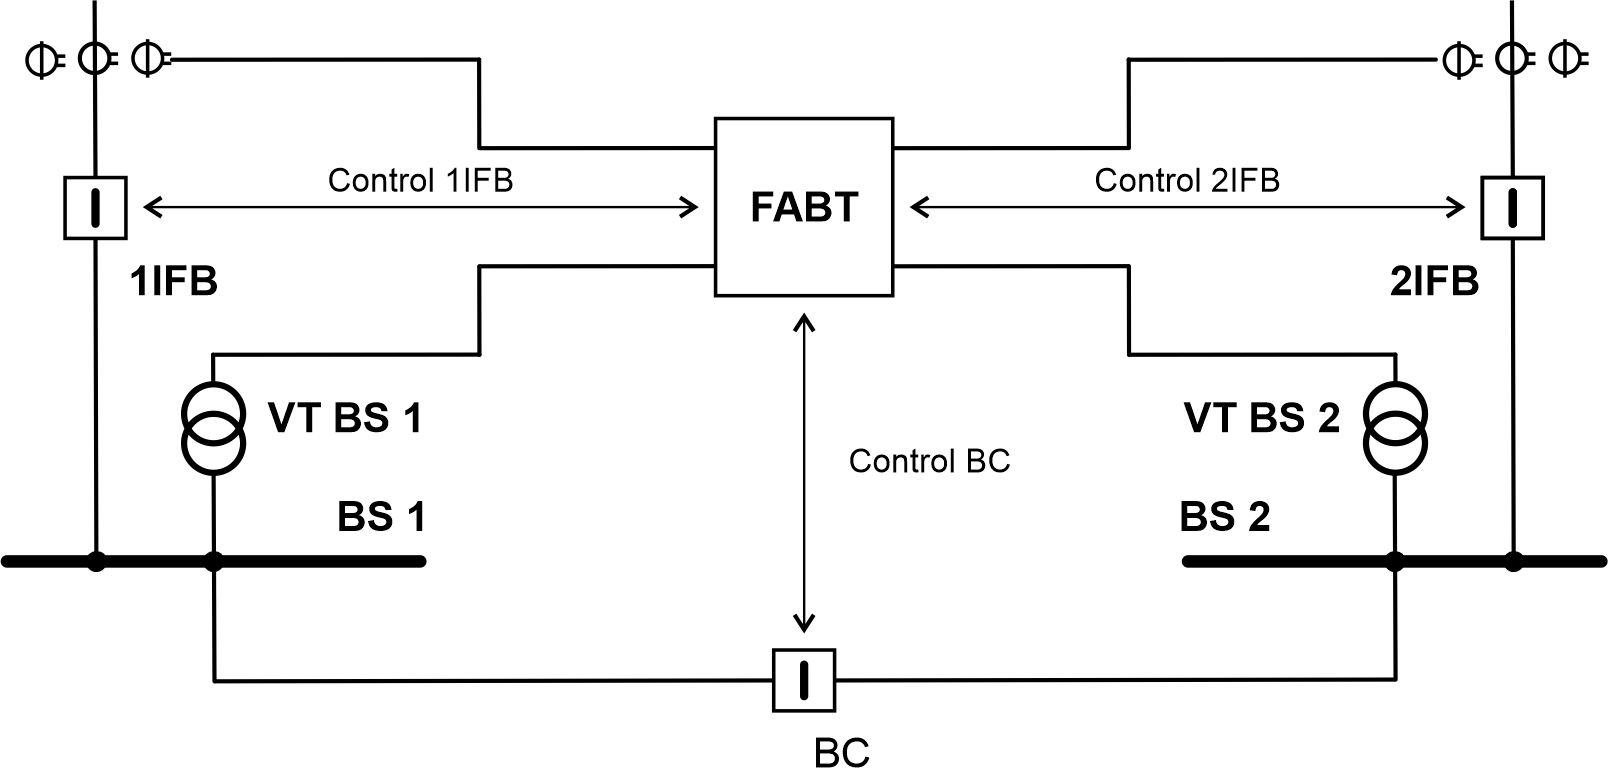
\includegraphics[width=\linewidth]{image1.png}
  \par\vspace{1mm}
  \textbf{а)}
  \commentnote{DISS-005-C0008}{Евдаков Алексей}{Перевести на русский}
\end{minipage}\hfill
\begin{minipage}{0.48\textwidth}
  \centering
  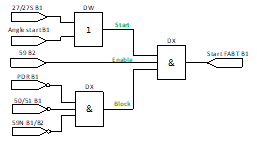
\includegraphics[width=\linewidth]{image2.png}
  \par\vspace{1mm}
  \textbf{б)}
\end{minipage}
\caption[Схемы а) подключения БАВР; б) логики срабатывания БАВР]{Схемы а) подключения БАВР; б) логики срабатывания БАВР\wordchoice{}{.}\wordrevnote{DISS-005-REV0001}{Евдаков Алексей}{2025-01-27}{вставка точки}}
\label{fig:bavr_schemes}
\end{figure}

% DISS-005-B0225
Использование этих базовых органов в алгоритмах БАВР обеспечивает практически мгновенную реакцию на аварию, что позволяет обеспечить~\cite{yablokov2022}:

\section{Фрагмент 2: Математические модели сигналов тока}

% DISS-005-B0778
В качестве входного сигнала использовался синусоидальный сигнал с апериодической составляющей, определяемой согласно первому закону коммутации о неразрывности тока (Ошибка! Источник ссылки не найден.), формула~\eqref{eq:kz_current}:
% DISS-005-B0779..B0781 (Таблица-обёртка формулы DISS-005-TAB-038)
\begin{equation}
\label{eq:kz_current}
i(t) = I_{\text{кз}} \cdot \sqrt{2} \cdot \left(\cos\phi_{\text{КЗ}} \cdot e^{-\frac{t}{\tau_0}} - \cos(\omega t + \phi_{\text{КЗ}})\right)
\end{equation}

% DISS-005-B0782
\noindent где $i(t)$~--- мгновенные значения сигнала тока, $I_{\text{кз}}$~--- амплитуда тока КЗ, $\phi_{\text{КЗ}}$~--- угол начала КЗ, $\tau_0$~--- постоянная времени затухания, $\omega = 2 \cdot \pi \cdot f$~--- угловая частота, $t$~--- время переходного процесса.

% DISS-005-B0783
Для катушек Роговского сигнал пропорционален производной первичного тока ($i'(t)$), формула~\eqref{eq:rogowski_derivative}:
% DISS-005-B0784..B0786 (Таблица-обёртка формулы DISS-005-TAB-039)
\begin{equation}
\label{eq:rogowski_derivative}
i'(t) = I_{\text{кз}} \cdot \sqrt{2} \cdot \left(-\frac{\cos\phi_{\text{КЗ}}}{\tau_0} \cdot e^{-\frac{t}{\tau_0}} + \omega \cdot \sin(\omega t + \phi_{\text{КЗ}})\right)
\end{equation}

\section{Фрагмент 3: Научная таблица параметров}

В табл.~\ref{tab:filter_settings} приведены рассчитанные параметры фильтрации для функции фильтрации «пустых» осциллограмм.

% DISS-005-B2012..B2038 (Научная таблица DISS-005-TAB-088)
\begin{table}[htbp]
\centering
\caption{Уставки для функции фильтрации «пустых» осциллограмм}
\label{tab:filter_settings}
\vspace{2mm}
\begin{tabular}{|l|l|c|c|c|}
\hline
\multicolumn{2}{|c|}{\textbf{сигнал}} & \textbf{\begin{tabular}[c]{@{}c@{}}Расхождение\\(delta)\end{tabular}} & \textbf{std\_dev} & \textbf{max\_abs} \\ \hline
\multirow{2}{*}{Нормализованные} & Ток & 0.1/20 & 0.05/20 & 0.005/20 \\ \cline{2-5} 
 & Напряжение & 0.05/3 & 0.025/3 & 0.05/3 \\ \hline
\multirow{2}{*}{Сырые} & Ток & 0.4 & 0.2 & Х \\ \cline{2-5} 
 & Напряжение & 0.05 & 0.025 & Х \\ \hline
\end{tabular}
\end{table}

% DISS-005-B2039
\noindent\small\textit{Примечание:} Нормализация проводится с учётом масштабирования базисов (умножением на коэффициенты 3 для напряжений и 20 для токов, см. раздел 3.5.2), поэтому уставки для нормализованных сигналов здесь представлены как доля от этих масштабированных базисов (т.е. поделены на эти коэффициенты)
\normalsize

\section{Проверка перекрёстных ссылок}
В данном документе проверена связность всех перекрёстных ссылок:
\begin{itemize}
  \item Ссылка на рисунок: рис.~\ref{fig:bavr_schemes} на с.~\pageref{fig:bavr_schemes};
  \item Ссылка на формулы: формулы~\eqref{eq:kz_current} и~\eqref{eq:rogowski_derivative} на с.~\pageref{eq:kz_current};
  \item Ссылка на таблицу: табл.~\ref{tab:filter_settings} на с.~\pageref{tab:filter_settings};
  \item Библиографическая ссылка: \cite{yablokov2022}.
\end{itemize}

\begin{thebibliography}{9}
\bibitem{yablokov2022}
Яблоков~А.~А., Евдаков~А.~Е. Применение методов машинного обучения для идентификации аварийных режимов в системах электроснабжения // Энергетика. Изв. высш. учеб. заведений и энерг. объединений СНГ. 2022.
\end{thebibliography}

\end{document}
